\documentclass[11pt,a4paper]{report}
\usepackage[textwidth=37em,vmargin=30mm]{geometry}
\usepackage{calc,xunicode,amsmath,amssymb,paralist,enumitem,tabu,booktabs,datetime2,xeCJK,xeCJKfntef,listings}
\usepackage{tocloft,fancyhdr,tcolorbox,xcolor,graphicx,eso-pic,xltxtra,xelatexemoji}

\newcommand{\envyear}[0]{2025}
\newcommand{\envdatestr}[0]{2025-02-21}
\newcommand{\envfinaldir}[0]{webdb/2025/20250221/final}

\usepackage[hidelinks]{hyperref}
\hypersetup{
    colorlinks=false,
    pdfpagemode=FullScreen,
    pdftitle={Web Digest - \envdatestr}
}

\setlength{\cftbeforechapskip}{10pt}
\renewcommand{\cftchapfont}{\rmfamily\bfseries\large\raggedright}
\setlength{\cftbeforesecskip}{2pt}
\renewcommand{\cftsecfont}{\sffamily\small\raggedright}

\setdefaultleftmargin{2em}{2em}{1em}{1em}{1em}{1em}

\usepackage{xeCJK,xeCJKfntef}
\xeCJKsetup{PunctStyle=plain,RubberPunctSkip=false,CJKglue=\strut\hskip 0pt plus 0.1em minus 0.05em,CJKecglue=\strut\hskip 0.22em plus 0.2em}
\XeTeXlinebreaklocale "zh"
\XeTeXlinebreakskip = 0pt


\setmainfont{Brygada 1918}
\setromanfont{Brygada 1918}
\setsansfont{IBM Plex Sans}
\setmonofont{JetBrains Mono NL}
\setCJKmainfont{Noto Serif CJK SC}
\setCJKromanfont{Noto Serif CJK SC}
\setCJKsansfont{Noto Sans CJK SC}
\setCJKmonofont{Noto Sans CJK SC}

\setlength{\parindent}{0pt}
\setlength{\parskip}{8pt}
\linespread{1.15}

\lstset{
	basicstyle=\ttfamily\footnotesize,
	numbersep=5pt,
	backgroundcolor=\color{black!5},
	showspaces=false,
	showstringspaces=false,
	showtabs=false,
	tabsize=2,
	captionpos=b,
	breaklines=true,
	breakatwhitespace=true,
	breakautoindent=true,
	linewidth=\textwidth
}






\newcommand{\coverpic}[2]{
    % argv: itemurl, authorname
    Cover photo by #2~~(\href{#1}{#1})
}
\newcommand{\makeheader}[0]{
    \begin{titlepage}
        % \newgeometry{hmargin=15mm,tmargin=21mm,bmargin=12mm}
        \begin{center}
            
            \rmfamily\scshape
            \fontspec{BaskervilleF}
            \fontspec{Old Standard}
            \fontsize{59pt}{70pt}\selectfont
            WEB\hfill DIGEST
            
            \vfill
            % \vskip 30pt
            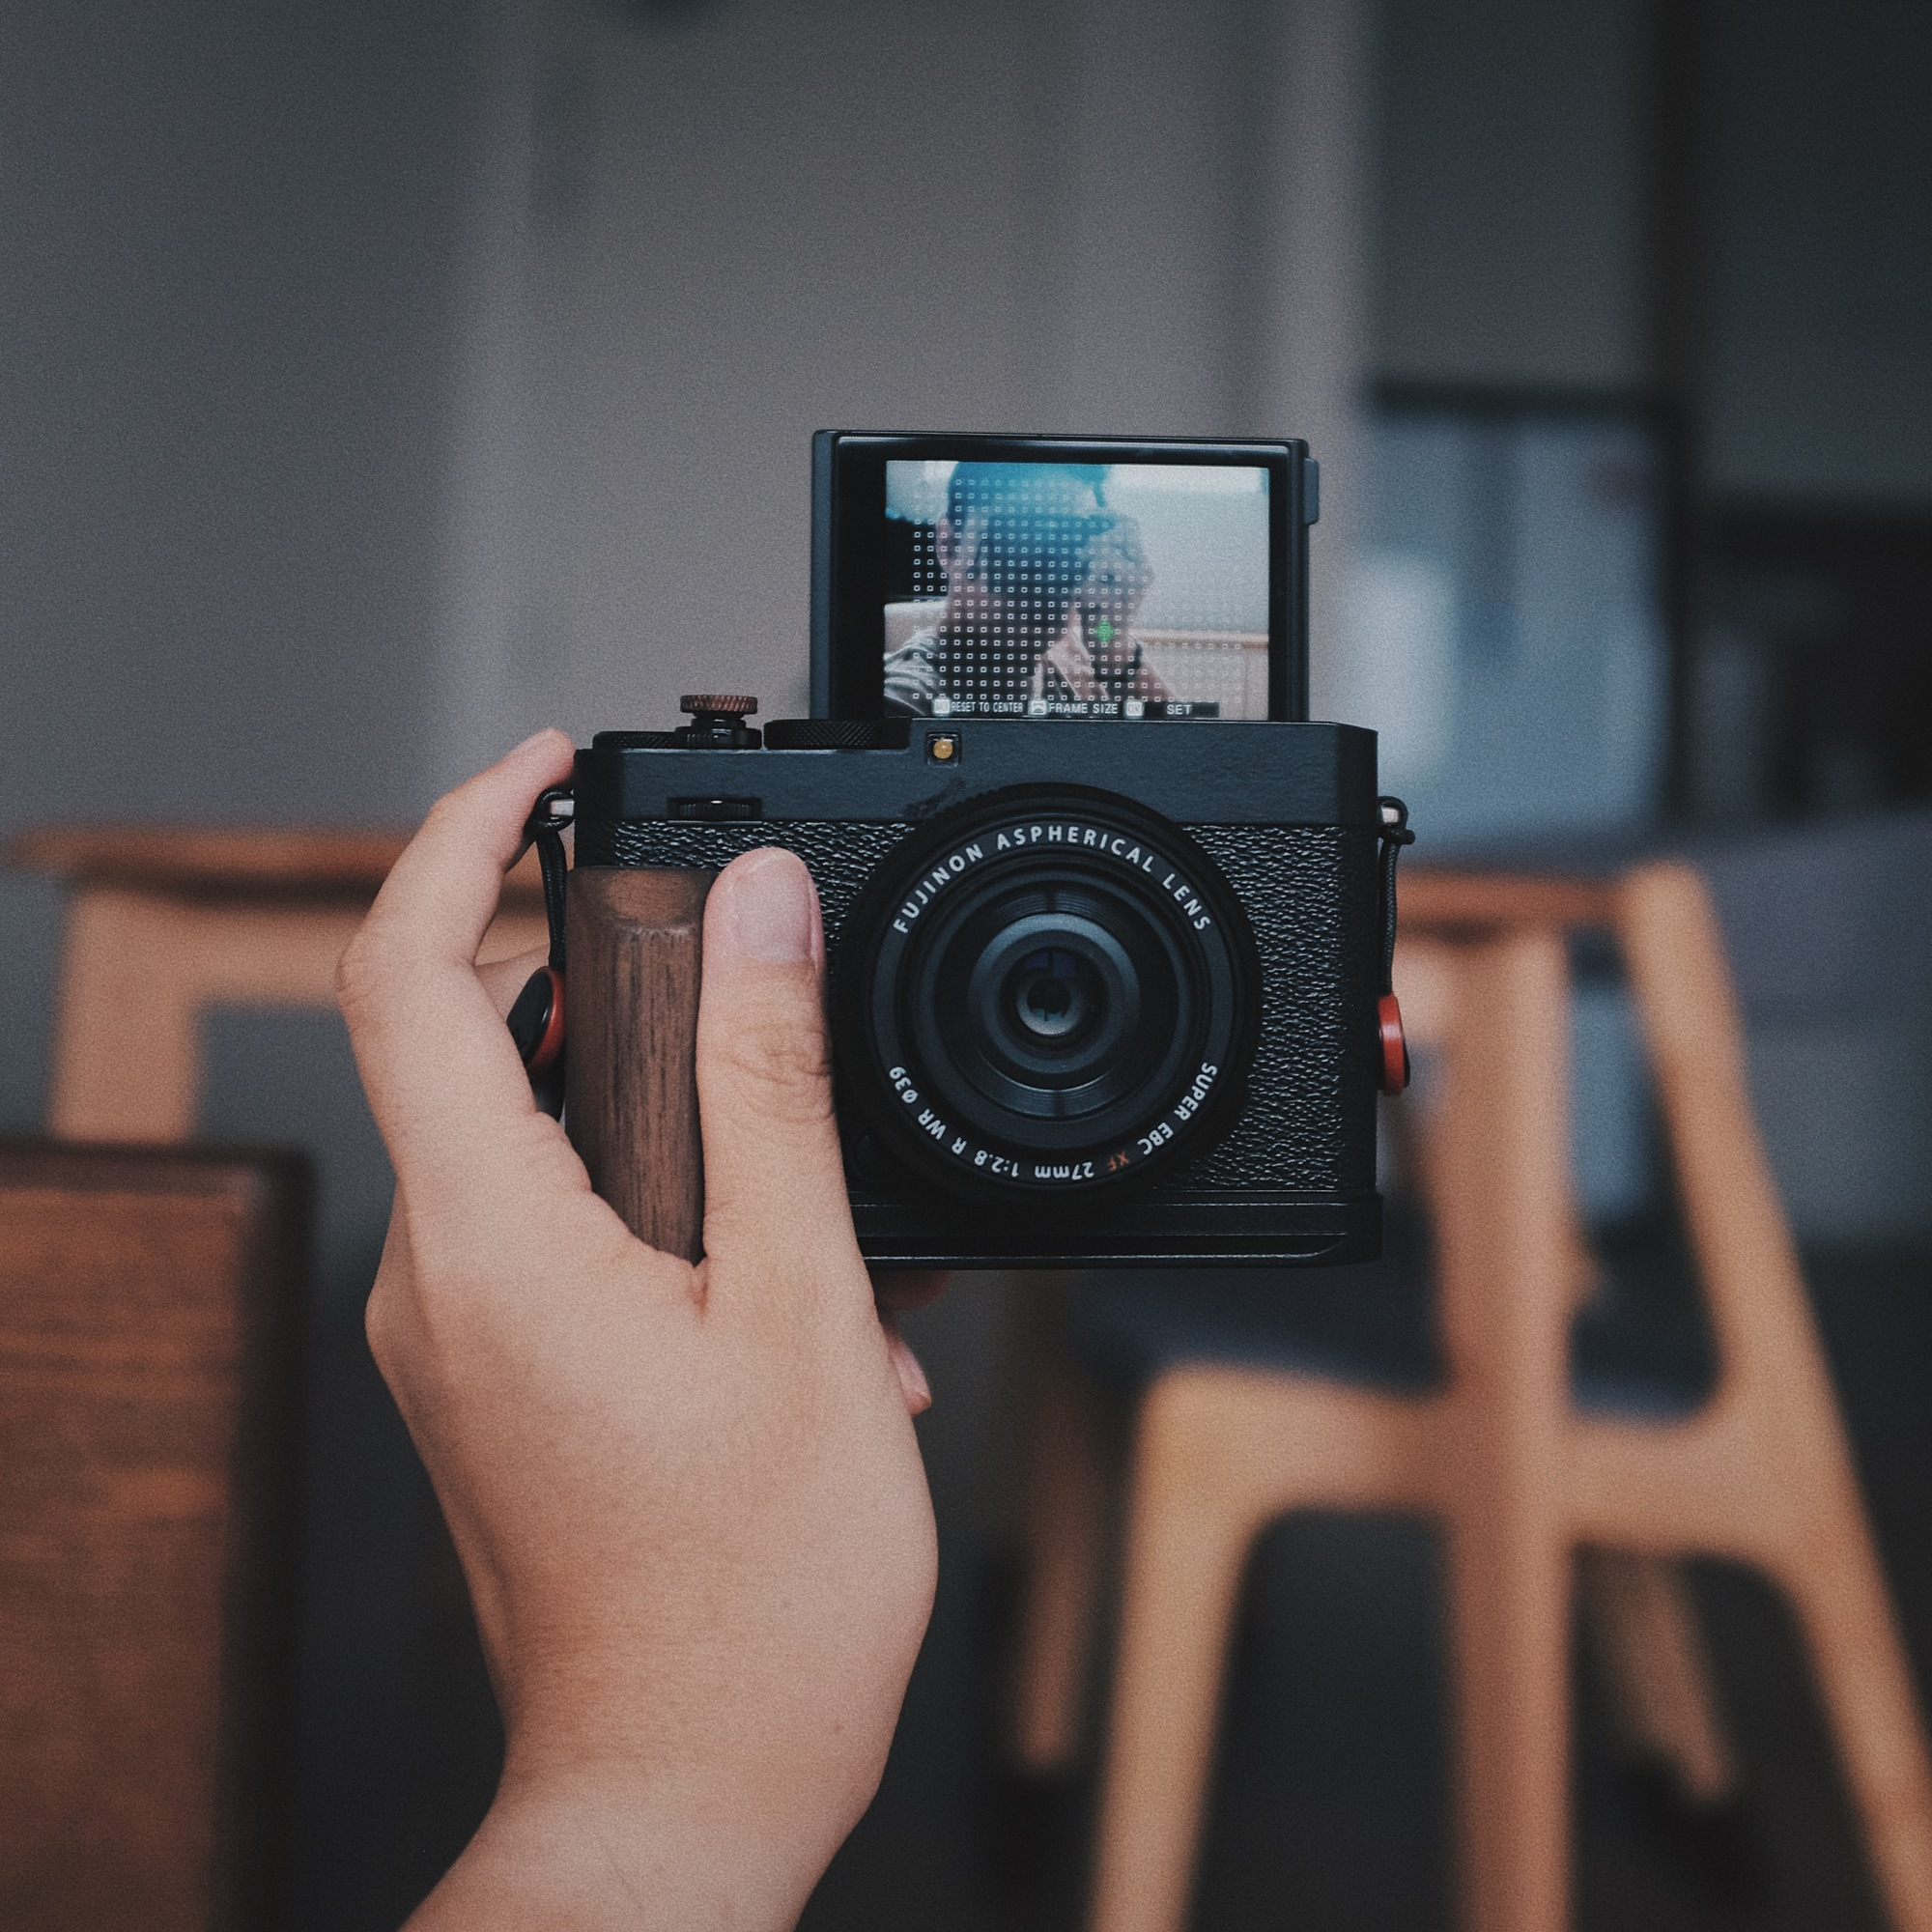
\includegraphics[width=\linewidth]{\envfinaldir/coverpic-prod.jpg}\par
            % \vskip 30pt
            \vfill

            \normalsize\rmfamily\scshape
            \copyright{} The Web Digest Project \hfill\large \envdatestr
        \end{center}
    \end{titlepage}
    % \restoregeometry
}
\newcommand{\simplehref}[1]{%
    \textcolor{blue!80!green}{\href{#1}{#1}}%
}
\renewcommand{\contentsname}{\center\Huge\sffamily\bfseries Contents\par\vskip 20pt}
\newcounter{ipartcounter}
\setcounter{ipartcounter}{0}
\newcommand{\ipart}[1]{
    % \vskip 20pt
    \clearpage
    \stepcounter{ipartcounter}
    \phantomsection
    \addcontentsline{toc}{chapter}{#1}
    % \begin{center}
    %     \Huge
    %     \sffamily\bfseries
    %     #1
    % \end{center}
    % \vskip 20pt plus 7pt
}
\newcounter{ichaptercounter}
\setcounter{ichaptercounter}{0}
\newcommand{\ichapter}[1]{
    % \vskip 20pt
    \clearpage
    \stepcounter{ichaptercounter}
    \phantomsection
    \addcontentsline{toc}{section}{\numberline{\arabic{ichaptercounter}}#1}
    \begin{center}
        \Huge
        \sffamily\bfseries
        #1
    \end{center}
    \vskip 20pt plus 7pt
}
\newcommand{\entrytitlefont}[1]{\subsection*{\raggedright\Large\sffamily\bfseries#1}}
\newcommand{\entryitemGeneric}[2]{
    % argv: title, url
    \parbox{\linewidth}{
        \entrytitlefont{#1}\par\vskip 5pt
        \footnotesize\ttfamily\mdseries
        \simplehref{#2}
    }\vskip 11pt plus 11pt minus 1pt
}
\newcommand{\entryitemGithub}[3]{
    % argv: title, url, desc
    \parbox{\linewidth}{
        \entrytitlefont{#1}\par\vskip 5pt
        \footnotesize\ttfamily\mdseries
        \simplehref{#2}\par\vskip 5pt
        \small\rmfamily\mdseries#3
    }\vskip 11pt plus 11pt minus 1pt
}
\newcommand{\entryitemAp}[3]{
    % argv: title, url, desc
    \parbox{\linewidth}{
        \entrytitlefont{#1}\par\vskip 5pt
        \footnotesize\ttfamily\mdseries
        \simplehref{#2}\par\vskip 5pt
        \small\rmfamily\mdseries#3
    }\vskip 11pt plus 11pt minus 1pt
}
\newcommand{\entryitemHackernews}[3]{
    % argv: title, hnurl, rawurl
    % \parbox{\linewidth}{
    %     \entrytitlefont{#1}\par\vskip 5pt
    %     \footnotesize\ttfamily\mdseries
    %     \simplehref{#3}\par
    %     \textcolor{black!50}{\href{#2}{#2}}
    % }\vskip 11pt plus 11pt minus 1pt
    \begin{minipage}{\linewidth}
            \entrytitlefont{#1}\par\vskip 5pt
            \footnotesize\ttfamily\mdseries
            \simplehref{#3}\par
            \textcolor{black!50}{\href{#2}{#2}}
    \end{minipage}\par\vskip 11pt plus 11pt minus 1pt
}







\begin{document}

\makeheader

\tableofcontents\clearpage




\ipart{Developers}
\ichapter{Hacker News}
\entryitemTwoLinks{Show HN: Immersive Gaussian Splat experience of Sutro Tower, San Francisco}{https://news.ycombinator.com/item?id=43120582}{https://vincentwoo.com/3d/sutro\_tower/}

\entryitemTwoLinks{DOGE puts \$1 spending limit on government employee credit cards}{https://news.ycombinator.com/item?id=43120231}{https://www.wired.com/story/doge-government-credit-cards/}

\entryitemTwoLinks{New horizons for Julia}{https://news.ycombinator.com/item?id=43118962}{https://lwn.net/Articles/1006117/}

\entryitemTwoLinks{OpenEuroLLM}{https://news.ycombinator.com/item?id=43118634}{https://openeurollm.eu/}

\entryitemTwoLinks{AWS S3 SDK breaks its compatible services}{https://news.ycombinator.com/item?id=43118592}{https://xuanwo.io/links/2025/02/aws\_s3\_sdk\_breaks\_its\_compatible\_services/}

\entryitemTwoLinks{You can't build a moat with AI (redux)}{https://news.ycombinator.com/item?id=43118512}{https://frontierai.substack.com/p/you-cant-build-a-moat-with-ai-redux}

\entryitemTwoLinks{Obsidian is now free for work}{https://news.ycombinator.com/item?id=43117020}{https://obsidian.md/blog/free-for-work/}

\entryitemTwoLinks{A cryptocurrency scam that turned a small town against itself}{https://news.ycombinator.com/item?id=43116410}{https://www.nytimes.com/2025/02/19/magazine/cryptocurrency-scam-kansas-heartland-bank.html}

\entryitemTwoLinks{Spice86 – A PC emulator for real mode reverse engineering}{https://news.ycombinator.com/item?id=43116112}{https://github.com/OpenRakis/Spice86}

\entryitemTwoLinks{Obsidian is now free for work}{https://news.ycombinator.com/item?id=43115767}{https://obsidian.md/pricing}

\entryitemTwoLinks{Helix: A vision-language-action model for generalist humanoid control}{https://news.ycombinator.com/item?id=43115079}{https://www.figure.ai/news/helix}

\entryitemTwoLinks{Texas banned abortion, then sepsis rates soared}{https://news.ycombinator.com/item?id=43114990}{https://www.propublica.org/article/texas-abortion-ban-sepsis-maternal-mortality-analysis}

\entryitemTwoLinks{Customizable HTML Select}{https://news.ycombinator.com/item?id=43113790}{https://developer.chrome.com/blog/rfc-customizable-select}

\entryitemTwoLinks{The Amazon Appstore for Android devices will be discontinued on August 20, 2025}{https://news.ycombinator.com/item?id=43113397}{https://www.amazon.com/gp/mas/appstore/android/faq}

\entryitemTwoLinks{After 20 years, math couple solves major group theory problem}{https://news.ycombinator.com/item?id=43113024}{https://www.quantamagazine.org/after-20-years-math-couple-solves-major-group-theory-problem-20250219/}

\entryitemTwoLinks{DOGE has 'god mode' access to government data}{https://news.ycombinator.com/item?id=43112084}{https://www.theatlantic.com/technology/archive/2025/02/doge-god-mode-access/681719/}

\entryitemTwoLinks{FAQ on Microsoft's topological qubit thing}{https://news.ycombinator.com/item?id=43112021}{https://scottaaronson.blog/?p=8669}

\entryitemTwoLinks{Grok 3: Another win for the bitter lesson}{https://news.ycombinator.com/item?id=43111963}{https://www.thealgorithmicbridge.com/p/grok-3-another-win-for-the-bitter}

\entryitemTwoLinks{Magma: A foundation model for multimodal AI agents}{https://news.ycombinator.com/item?id=43110265}{https://microsoft.github.io/Magma/}

\entryitemTwoLinks{Mexico issues legal threat to Google}{https://news.ycombinator.com/item?id=43110226}{https://thecomeback.com/politics/mexico-legal-action-donald-trump-executive-order.html}\ichapter{Phoronix}
\entryitemGeneric{\hskip 0pt{}Mesa's Zink Driver Enables cl\_khr\_gl\_sharing, Working On DaVinci Resolve Support}{https://www.phoronix.com/news/Zink-cl\_khr\_gl\_sharing}

\entryitemGeneric{\hskip 0pt{}Rust 1.85 Release Stabilizes Rust 2024 Edition}{https://www.phoronix.com/news/Rust-1.85-Released}

\entryitemGeneric{\hskip 0pt{}OpenRazer 3.10 Delivers New Razer Hardware Support For Linux Users}{https://www.phoronix.com/news/OpenRazer-3.10-Released}

\entryitemGeneric{\hskip 0pt{}Linux Finally Introducing A Standardized Way Of Informing User-Space Over Hung GPUs}{https://www.phoronix.com/news/Linux-6.14-Wedged-GPUs-User}

\entryitemGeneric{\hskip 0pt{}Ubuntu 24.04.2 LTS Now Available With Initial HWE Stack}{https://www.phoronix.com/news/Ubuntu-24.04.2-LTS}

\entryitemGeneric{\hskip 0pt{}Linux Lazy Unmap Flush "LUF" Reducing TLB Shootdowns By 97\%, Faster AI LLM Performance}{https://www.phoronix.com/news/Linux-Lazy-Unmap-Flush}

\entryitemGeneric{\hskip 0pt{}New Patches Would Make All Kernel Encryption/Decryption Faster On x86/x86\_64 Hardware}{https://www.phoronix.com/news/Linux-x86-Crypt-Drop-Fallback}

\entryitemGeneric{\hskip 0pt{}Debian Policy Updated With New Packaging Guidance \& Updated Chinese Translations}{https://www.phoronix.com/news/Debian-Policy-New-Guidance}

\entryitemGeneric{\hskip 0pt{}GNOME Mutter Adds Debug Option To Override Multi-GPU Copy Mode}{https://www.phoronix.com/news/GNOME-Mutter-Debug-Copy-Mode}\ichapter{Dribbble}
\entryitemGeneric{\hskip 0pt{}Puzzle Fintech Website Design [Case Study]}{https://dribbble.com/shots/25478108-Puzzle-Fintech-Website-Design-Case-Study}

\entryitemGeneric{\hskip 0pt{}Sugar Glider Logo}{https://dribbble.com/shots/25653559-Sugar-Glider-Logo}

\entryitemGeneric{\hskip 0pt{}Pendleton Whisky}{https://dribbble.com/shots/25650439-Pendleton-Whisky}

\entryitemGeneric{\hskip 0pt{}Logo Design for Ai Assistant Part One}{https://dribbble.com/shots/25652926-Logo-Design-for-Ai-Assistant-Part-One}

\entryitemGeneric{\hskip 0pt{}Cimet Software Business Cards}{https://dribbble.com/shots/25648529-Cimet-Software-Business-Cards}

\entryitemGeneric{\hskip 0pt{}Fintech UI Design}{https://dribbble.com/shots/25647596-Fintech-UI-Design}

\entryitemGeneric{\hskip 0pt{}Enso Homes Logomark}{https://dribbble.com/shots/25632132-Enso-Homes-Logomark}

\entryitemGeneric{\hskip 0pt{}Flextro - Logo Design Update}{https://dribbble.com/shots/25648485-Flextro-Logo-Design-Update}

\entryitemGeneric{\hskip 0pt{}Reign - Logotype Design}{https://dribbble.com/shots/25639247-Reign-Logotype-Design}

\entryitemGeneric{\hskip 0pt{}E + Chart Logo Animation}{https://dribbble.com/shots/25640702-E-Chart-Logo-Animation}

\entryitemGeneric{\hskip 0pt{}Pigeon}{https://dribbble.com/shots/25641861-Pigeon}

\entryitemGeneric{\hskip 0pt{}Minimalist S Logo // For Sale}{https://dribbble.com/shots/25641404-Minimalist-S-Logo-For-Sale}

\entryitemGeneric{\hskip 0pt{}Smart Home Hub}{https://dribbble.com/shots/25637672-Smart-Home-Hub}

\entryitemGeneric{\hskip 0pt{}Recruitment Dashboard}{https://dribbble.com/shots/25605862-Recruitment-Dashboard}

\entryitemGeneric{\hskip 0pt{}Lume responsive}{https://dribbble.com/shots/25638482-Lume-responsive}

\entryitemGeneric{\hskip 0pt{}Mobile App for a Wellbeing Product ✦ Routine Hero}{https://dribbble.com/shots/25640481-Mobile-App-for-a-Wellbeing-Product-Routine-Hero}

\entryitemGeneric{\hskip 0pt{}Form Golf Monogram}{https://dribbble.com/shots/25643873-Form-Golf-Monogram}

\entryitemGeneric{\hskip 0pt{}Oh Baby!!}{https://dribbble.com/shots/25630659-Oh-Baby}

\entryitemGeneric{\hskip 0pt{}Alpaca}{https://dribbble.com/shots/25627851-Alpaca}

\entryitemGeneric{\hskip 0pt{}Cupid}{https://dribbble.com/shots/25629698-Cupid}

\entryitemGeneric{\hskip 0pt{}Happy Valentine's Day}{https://dribbble.com/shots/25629557-Happy-Valentine-s-Day}

\entryitemGeneric{\hskip 0pt{}KOVEX - Logo Design}{https://dribbble.com/shots/25630984-KOVEX-Logo-Design}

\entryitemGeneric{\hskip 0pt{}Flows Lab UX/UI design}{https://dribbble.com/shots/25629797-Flows-Lab-UX-UI-design}

\entryitemGeneric{\hskip 0pt{}Speed Test App Design}{https://dribbble.com/shots/25627991-Speed-Test-App-Design}


\ipart{Developers~~~~(zh-Hans)}
\ichapter{Solidot}
\entryitemGeneric{\hskip 0pt{}研究发现手机断网有助于改进心理健康}{https://www.solidot.org/story?sid=80608}

\entryitemGeneric{\hskip 0pt{}亚马逊将于 8 月 20 日关闭 Android Appstore }{https://www.solidot.org/story?sid=80607}

\entryitemGeneric{\hskip 0pt{}因关税宏碁将对美国销售的笔记本电脑产品提价 10\%}{https://www.solidot.org/story?sid=80606}

\entryitemGeneric{\hskip 0pt{}Pi-hole v6 释出}{https://www.solidot.org/story?sid=80605}

\entryitemGeneric{\hskip 0pt{}法国 WEST 托卡马克核聚装置维持等离子体运行 22 分钟}{https://www.solidot.org/story?sid=80604}

\entryitemGeneric{\hskip 0pt{}小行星 2024 YR4 撞击地球概率下调}{https://www.solidot.org/story?sid=80603}

\entryitemGeneric{\hskip 0pt{}从 2000-2023 年全球冰川缩小 了5\% 以上}{https://www.solidot.org/story?sid=80602}

\entryitemGeneric{\hskip 0pt{}微软宣布其首款量子芯片 Majorana 1 }{https://www.solidot.org/story?sid=80601}

\entryitemGeneric{\hskip 0pt{}微软将记事本的 AI 重写功能藏于付费墙内}{https://www.solidot.org/story?sid=80600}

\entryitemGeneric{\hskip 0pt{}惠普收购 Humane 资产,其 AI 产品 AI Pins 将在 10 天内停止工作}{https://www.solidot.org/story?sid=80599}

\entryitemGeneric{\hskip 0pt{}为遵守欧洲隐私法规微软将为欧洲用户移除多项 Windows 文件管理器功能}{https://www.solidot.org/story?sid=80598}

\entryitemGeneric{\hskip 0pt{}中国科学家的锂离子修复技术能延寿六倍}{https://www.solidot.org/story?sid=80597}

\entryitemGeneric{\hskip 0pt{}27\% 的 CFO 职位招聘描述提及 AI }{https://www.solidot.org/story?sid=80596}

\entryitemGeneric{\hskip 0pt{}全球暖化可能导致城市鼠患}{https://www.solidot.org/story?sid=80595}

\entryitemGeneric{\hskip 0pt{}黑客在 Steam 游戏中植入恶意程序窃取玩家敏感数据}{https://www.solidot.org/story?sid=80594}

\entryitemGeneric{\hskip 0pt{}内核维护者称 Linus Torvalds 会不顾他们的反对意见合并 Rust 代码}{https://www.solidot.org/story?sid=80593}

\entryitemGeneric{\hskip 0pt{}Valve 公开《团队要塞2》 SDK}{https://www.solidot.org/story?sid=80592}

\entryitemGeneric{\hskip 0pt{}Niantic 考虑向沙特系企业出售《精灵宝可梦GO》}{https://www.solidot.org/story?sid=80591}

\entryitemGeneric{\hskip 0pt{}美国报业巨头用修辞避免提及勒索软件}{https://www.solidot.org/story?sid=80590}

\entryitemGeneric{\hskip 0pt{}欧洲预期寿命增长停滞}{https://www.solidot.org/story?sid=80589}


\ipart{Generic News}
\ichapter{AP News}
\entryitemWithDescription{\hskip 0pt{}What to know about Fort Knox's gold depository}{https://apnews.com/article/338bebb56885c142feaa0ff383c9ba37}{}

\entryitemWithDescription{\hskip 0pt{}Scottish Highland bull on the loose in Connecticut's rural hill country}{https://apnews.com/article/436b8ae25103fd281aa087ce4f0baeb3}{}

\entryitemWithDescription{\hskip 0pt{}Amazon MGM takes creative reins of James Bond, ending an era of family control of 007}{https://apnews.com/article/62db8105bb262e5bbea11b16e2edd9f2}{}

\entryitemWithDescription{\hskip 0pt{}Walmart rolled through 2024, but uncertainty about consumers and tariffs seep into year ahead}{https://apnews.com/article/b1404b671b10ff378887acd28c2d2140}{}

\entryitemWithDescription{\hskip 0pt{}Trump wants to know if there's gold in Fort Knox. (There is)}{https://apnews.com/article/f84f9f473d0551e7b055363e58f85759}{}

\entryitemWithDescription{\hskip 0pt{}Ex-Spain soccer boss Rubiales found guilty of sexual assault and fined for World Cup kiss}{https://apnews.com/article/184c72358cca4d4f94497c4e14333986}{}

\entryitemWithDescription{\hskip 0pt{}In its 10th episode, Kilauea, one of the world's most active volcanoes, is again spewing lava}{https://apnews.com/article/4bd3a5537ef821cff2f7bcf4eae94733}{}

\entryitemWithDescription{\hskip 0pt{}Can sandals be art? Birkenstock says yes, but a German court says no}{https://apnews.com/article/e3985066da164cffd2a0248e0c9b6675}{}

\entryitemWithDescription{\hskip 0pt{}Apple unveils a souped-up and more expensive version of its lowest priced iPhone}{https://apnews.com/article/1fc43f8b839d7995763fbe939f5de290}{}

\entryitemWithDescription{\hskip 0pt{}What's going on with the Kennedy Center under Trump?}{https://apnews.com/article/4305e2c3d5611c4bfb1686d597727369}{}

\entryitemWithDescription{\hskip 0pt{}U.S. and Canada want to put the new Cold War on ice and play a 4 Nations hockey final for the ages}{https://apnews.com/article/4572427a14a8e2b0365b5f6cfef28216}{}

\entryitemWithDescription{\hskip 0pt{}Historic ocean liner departs Philadelphia on voyage to become the world's largest artificial reef}{https://apnews.com/article/818c44d7f3078c4ffa3b8aa39f3329ed}{}

\entryitemWithDescription{\hskip 0pt{}Seven Chilean men are charged with burglarizing the homes of Mahomes, Burrow and other star athletes}{https://apnews.com/article/3c8b707fa21edc5d31285d88d6d80253}{}






\clearpage
\leavevmode\vfill
\footnotesize

Copyright \copyright{} 2023-2025 Neruthes and other contributors.

This document is published with CC BY-NC-ND 4.0 license.

The entries listed in this newsletter may be copyrighted by their respective creators.

This newsletter is generated by the Web Digest project.

The newsletters are also delivered via Telegram channel \CJKunderline{\href{https://t.me/webdigestchannel}{https://t.me/webdigestchannel}}.\\
RSS feed is available at \CJKunderline{\href{https://webdigest.pages.dev/rss.xml}{https://webdigest.pages.dev/rss.xml}}.

This newsletter is available in PDF at
\CJKunderline{\href{https://webdigest.pages.dev/}{https://webdigest.pages.dev/}}.

The source code being used to generate this newsletter is available at\\
\CJKunderline{\href{https://github.com/neruthes/webdigest}{https://github.com/neruthes/webdigest}}.

This newsletter is also available in
\CJKunderline{\href{http://webdigest.pages.dev/readhtml/\envyear/WebDigest-20250221.html}{HTML}} and
\CJKunderline{\href{https://github.com/neruthes/webdigest/blob/master/markdown/\envyear/WebDigest-20250221.md}{Markdown}}.


\coverpic{https://unsplash.com/photos/a-person-sitting-on-a-bed-in-a-room-RiFW3Von\_as}{Samir Vanegas}


\end{document}
